\section{Introduction}

%In connectomics, neuroscientists annotate neurons and their connectivity within 3D volumes to gain insight into the functional structure of the brain. Rapid progress in automatic sample preparation and electron microscopy (EM) acquisition techniques has made it possible to image large volumes of brain tissue at $\approx4\, nm$ per pixel to identify cells, synapses, and vesicles. For $40\, nm$ thick sections, a $1\, mm^3$ volume of brain contains $10^{15}$ voxels, or 1 petabyte of data. With so much data, manual annotation is infeasible, and automatic annotation methods are needed~\cite{jain2010,Liu2014,GALA2014,kaynig2015large}.

%Automatic annotation by segmentation and classification of brain tissue is challenging~\cite{isbi_challenge}. The state of the art uses supervised learning with convolutional neural networks~\cite{Ciresan:2012f}, or potentially even unsupervised learning~\cite{BogovicHJ13}. Typically, cell membranes are detected in 2D images, and the resulting region segmentation is grouped into geometrically-consistent cells across registered sections. Cells may also be segmented across registered sections in 3D directly. Using dynamic programming techniques~\cite{Masci:2013a} and a GPU cluster, these classifiers can segment $\approx1$ terabyte of data per hour ~\cite{kasthuri2015saturated}. This is sufficient to keep up with the 2D data capture process on state-of-the-art electron microscopes (though 3D registration is still an expensive offline operation).

In connectomics, neuroscientists annotate neurons and their connectivity within
3D volumes to gain insight into the functional structure of the brain. Rapid
progress in automatic sample preparation and electron microscopy (EM)
acquisition techniques has made it possible to image large volumes of brain
tissue at nanometer resolution. With a voxel size of
$4\times4\times40~\text{nm}^3$, a cubic millimeter volume is one petabyte of
data. With so much data, manual annotation is not feasible, and automatic
annotation methods are needed~\cite{jain2010,Liu2014,GALA2014,kaynig2015large}.

Automatic annotation by segmentation and classification of brain tissue is
challenging~\cite{isbi_challenge} and all available methods make errors, so 
the results must be \emph{proofread} by humans. This crucial
task serves two purposes: 1) to correct errors in the segmentation, and 2) to
increase the body of labeled data from which to train better automatic
segmentation methods. Recent proofreading tools provide intuitive user
interfaces to browse segmentation data in 2D and 3D and to identify and manually
correct errors~\cite{markus_proofreading,raveler,mojo2,haehn_dojo_2014}. Many
kinds of errors exist, such as inaccurate boundaries, but the most common are
\emph{split errors}, where a single segment is labeled as two, and \emph{merge
errors}, where two segments are labeled as one
(Fig.~\ref{fig:merge_and_slit_errors}). With user interaction, split errors can
be joined, and the missing boundary in a merge error can be defined with
manually-seeded watersheds~\cite{haehn_dojo_2014}. However, the visual
inspection to find errors takes the majority of the time, even with
semi-automatic correction tools~\cite{proofreading_bottleneck}.

\begin{figure}[t]
\begin{center}
  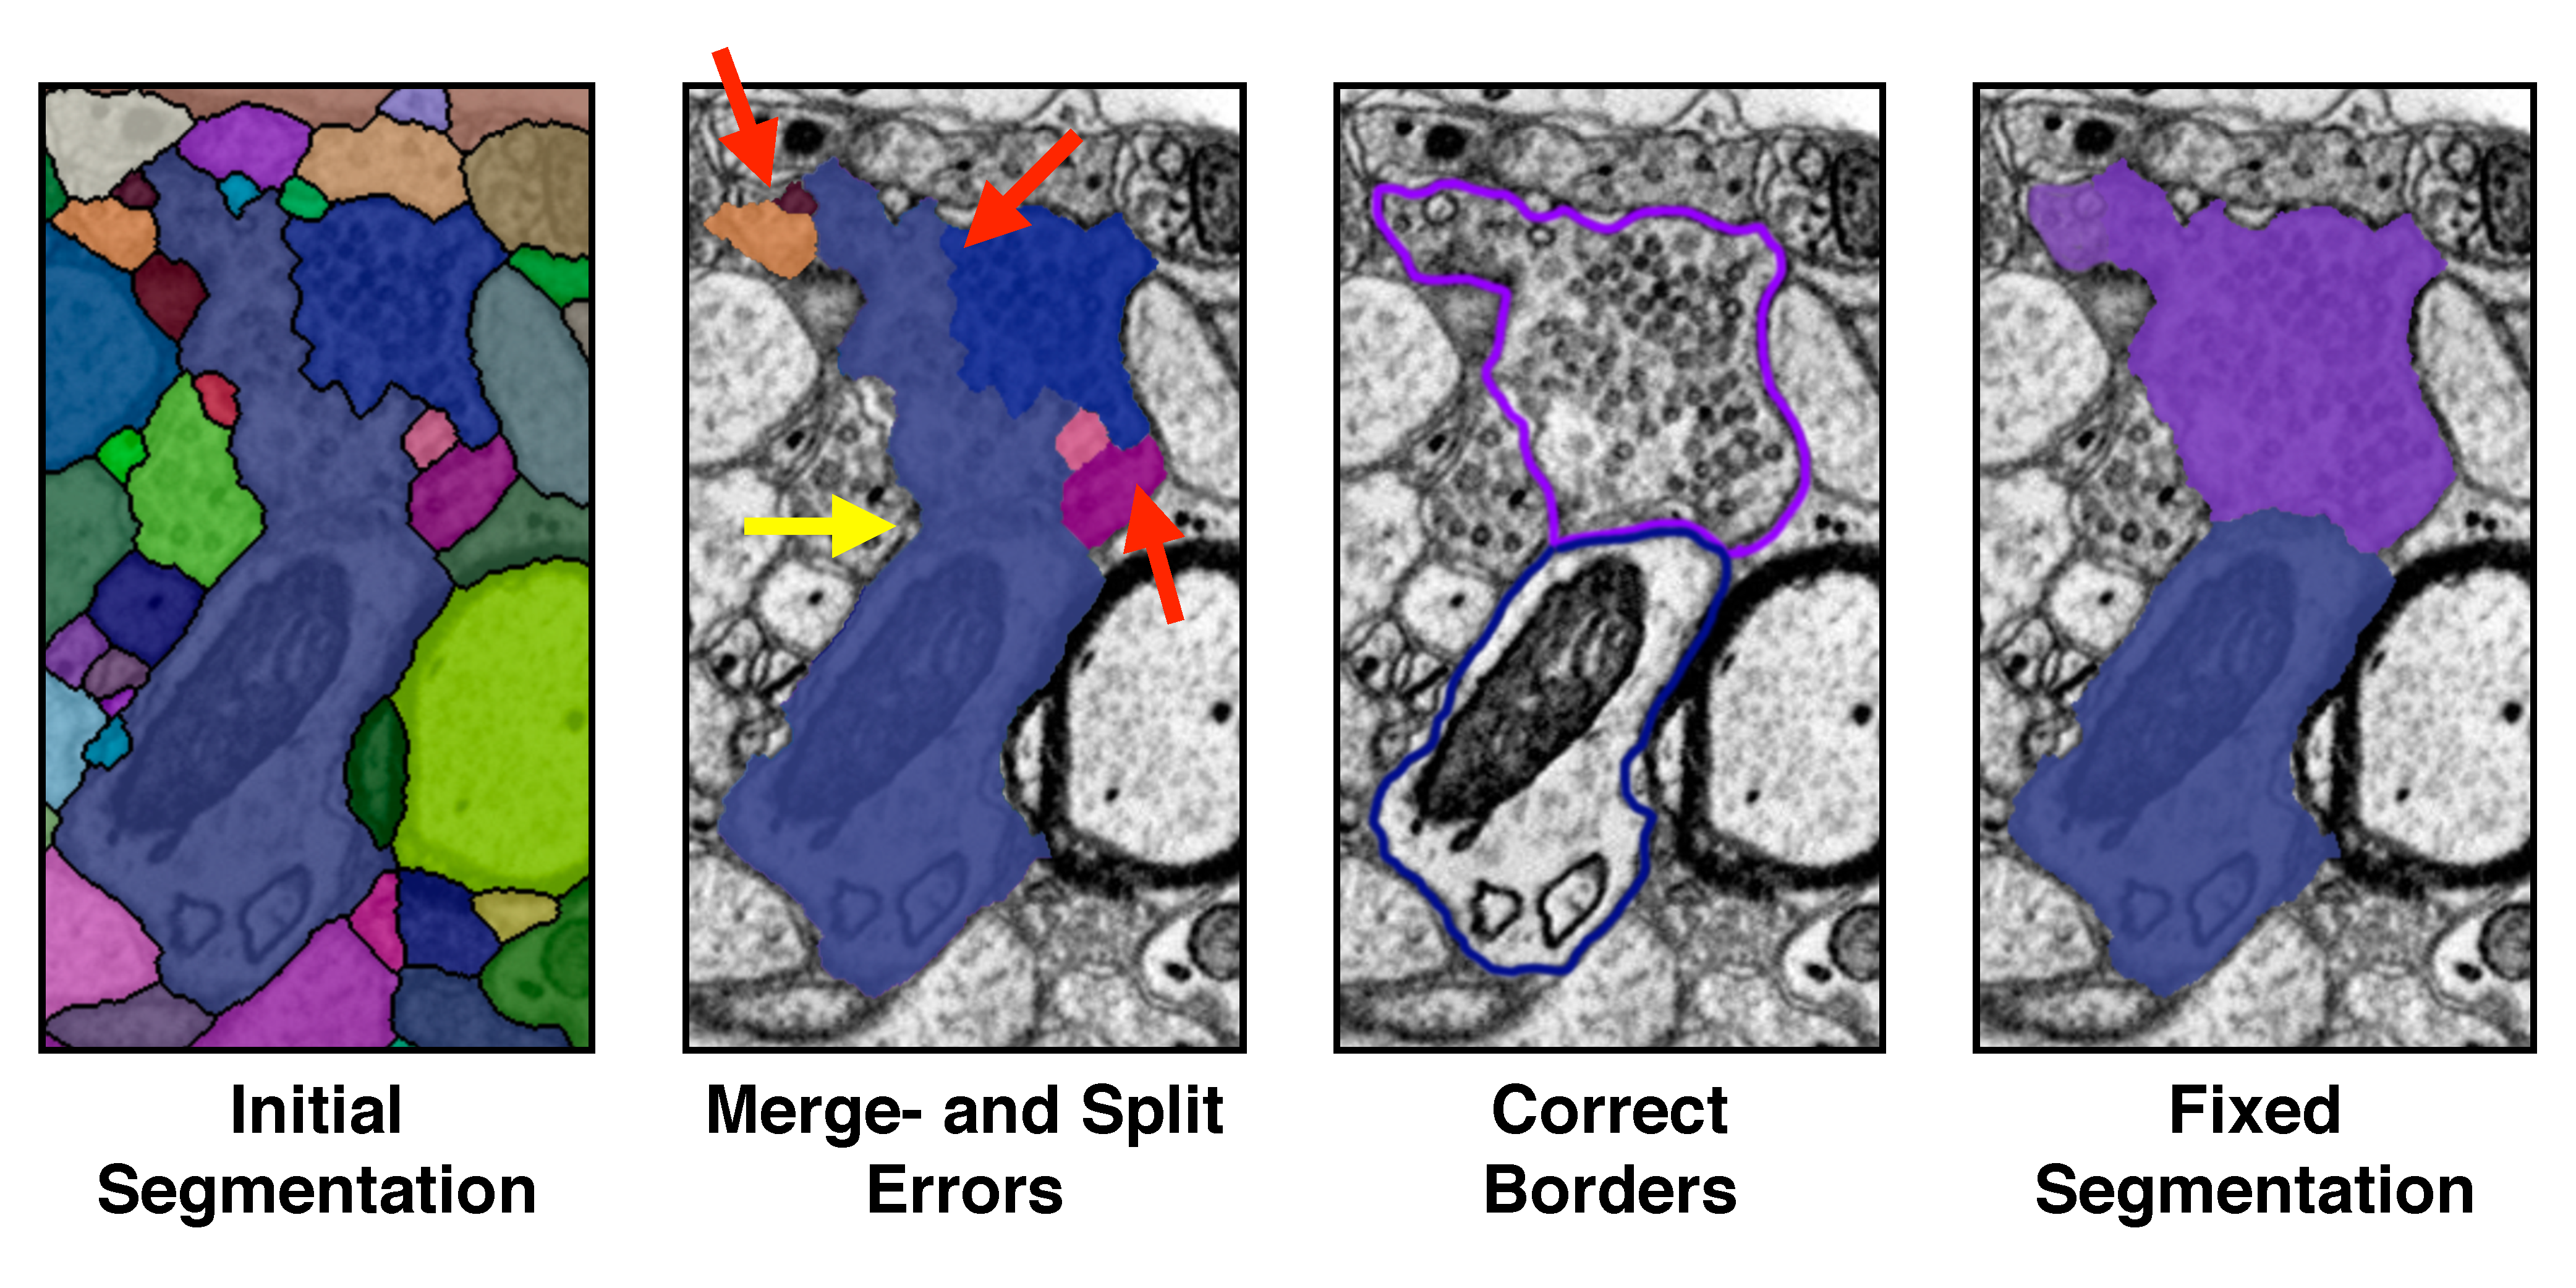
\includegraphics[width=\linewidth]{gfx/merge_and_split_errors.pdf}
\end{center}
\vspace{-4mm}
   \caption{The most common proofreading corrections are fixing split errors (red arrows) and merge errors (yellow arrow). A fixed segmentation matches the cell borders.}
   \vspace{-4mm}
\label{fig:merge_and_slit_errors}
\end{figure}

Our goal is to automatically detect potential split and merge errors to reduce visual
inspection time. Further, to reduce correction time, we propose
corrections to the user to accept or reject. We call this process \textit{guided
proofreading}.

We train a classifier for split error detection with a convolutional neural network
(CNN). This takes as input patches of membrane segmentation probabilities, cell
segmentation masks, and boundary masks, and outputs a split-probability score. As we
must process large data, this classifier only operates on cell boundaries, which
reduces computation over methods that analyze every pixel. For merge errors, we
invert and reuse the split classification network, and ask it to rate a
set of generated boundaries that hypothesize a split. %We compute
%corrections for both types of errors.

Possible erroneous regions are sorted by their score, and a candidate correction is generated for each
region. Then, a user works through this list of regions and corrections. In a
forced choice setting, the user either selects a correction or skips it to
advance to the next region. In an automatic setting, errors with a high probability are automatically corrected first, given an appropriate
probability threshold, after which the user would take over. Finally, to test
the limits of performance, we create an oracle which only accepts corrections
that improve the segmentation, based on knowledge of the ground truth. This is
guided proofreading with a perfect user.

We evaluate these methods on multiple connectomics datasets. For the forced
choice setting, we perform a quantitative user study with 20 novice users who
have no previous experience of proofreading EM data. We ask participants to
proofread a small segmentation volume in a fixed time frame. In a
between-subjects design, we compare guided proofreading to the semi-automatic
\textit{focused proofreading} approach by Plaza~\cite{focused_proofreading}. In
addition, we compare against the manual interactive proofreading tool
\textit{Dojo} by Haehn~\etal~\cite{haehn_dojo_2014}. We also asked four domain
experts to use guided proofreading and focused proofreading for comparison.

This paper makes the following contributions.
%
First, we present a CNN-based boundary classifier for split errors, plus a merge
error classifier that inverts the split error classifier. This proposes merge error corrections, 
which removes the need to manually draw the missing
edge. These classifiers automatically reduce error with little training data, which is expensive to collect for connectomics data.
%
Second, we develop a human-guided proofreading approach to correcting segmentation
volumes, and compare forced-choice interaction with
automatic and oracle proofreading.
%
Third, we present results of a quantitative user study assessing
guided proofreading. Our method is able to reduce segmentation
error faster than state-of-the-art semi-automatic tools for both novice and
expert users.
%
Fourth, we present the first connectomics proofreading benchmark, with image, label, and human interaction data, and evaluation code.

Guided proofreading is applicable to all existing automatic segmentation methods that produce a label map.
While we train models based on traditional CNN architectures, we propose an error correction approach with human interaction that works with many classifiers.
As such, we believe that our approach is a promising direction to proofread segmentations more efficiently and better tackle large volumes of connectomics imagery.

%Our goal is to add automatic detection of split and merge errors to proofreading tools. We design automatic classifiers that detect split and merge errors in segmentations so the user does not need to visually inspect the whole data volume to spot errors. A proofreading tool then recommends regions with a high probability of an error to the user, and suggest corrections to accept or reject. We call this process \textit{guided proofreading}.
%
%In this paper, we introduce classifiers to detect merge- and split errors based on a convolutional neural network (CNN). We believe that this is the first time that deep learning is applied to the task of proofreading. Our classifiers work on top of any existing automatic segmentation method to find potential errors and suggest corrections. Given a membrane segmentation from a fast automatic method, our classifiers operate on the boundaries of whole cell regions. Compared to techniques that must analyze every input pixel, we reduce the data analysis to the boundaries. First, we train a CNN to detect only split errors. The output of this network is a probability whether a boundary between two segments is valid or not. We then reuse the same network to also detect merge errors by generating possible boundaries within a cell and inverting the split error score. We create corrections for both types of errors which can be accepted or rejected. This reduces the proofreading operation to simple yes/no decisions.
%
%We further propose a greedy algorithm to perform proofreading. Possible erroneous regions are sorted by their score and the algorithm iteratively suggests a correction for each region. A user then works through this stream of regions and corrections. In a forced choice setting, the user either selects a correction or skips it to advance to the next region. This choice can be also performed automatically by running the algorithm until a configurable threshold is reached. In addition, if ground truth data is available, we can use a selection oracle to drive the forced choice selection. The oracle only accepts corrections which improve the automatic segmentation. This equals perfect proofreading.
%
%We evaluate our method automatically by threshold and oracle on multiple real-world connectomics datasets. To evaluate the forced choice setting, we perform a quantitative user study. The study targets non-experts with no previous experience of proofreading electron microscopy data. We ask the participants to proofread a small segmentation volume in a fixed time frame by performing yes/no decisions. The user study is designed as a between-subjects experiment and compares guided proofreading against two other methods: a recently published fully interactive proofreading tool named \textit{Dojo} by Haehn~\etal~\cite{haehn_dojo_2014} and the semi-automatic \textit{focused proofreading} approach by Plaza~\cite{focused_proofreading}. We also asked four domain experts to use guided proofreading and focused proofreading for additional comparison.
%
%Our first contribution is a classifier for split error detection based on a convolutional neural network. The classifier performs well even when trained with little amounts of training data. This is important since generating ground truth labels in connectomics requires manually labeling pixels and is very time-consuming. Our second contribution is a mechanism to identify merge-errors by re-using the split error classifier. Merge errors are usually less common than split errors in the oversegmented automatic labelings. However, they require more interaction during correction since split lines need to be manually drawn. Our method reduces this to a single click by providing the potential correction. The split and merge error identification is executed as a greedy algorithm to correct segmentation volumes, the third contribution of this paper. The algorithm can be driven automatically with a threshold, by an oracle based on ground truth and interactively in a forced choice setting. Our final contribution is our quantitative user study. We present statistically significant results showing that novice and expert users of guided proofreading are able to proofread a given dataset better and faster than with existing interactive and semi-automatic proofreading tools. As a consequence, we are able to provide tools to proofread segmentations more efficiently, and so better tackle large volumes of connectomics imagery.
